\documentclass{standalone}
\usepackage{tikz}
\usetikzlibrary{patterns, positioning}


\begin{document}
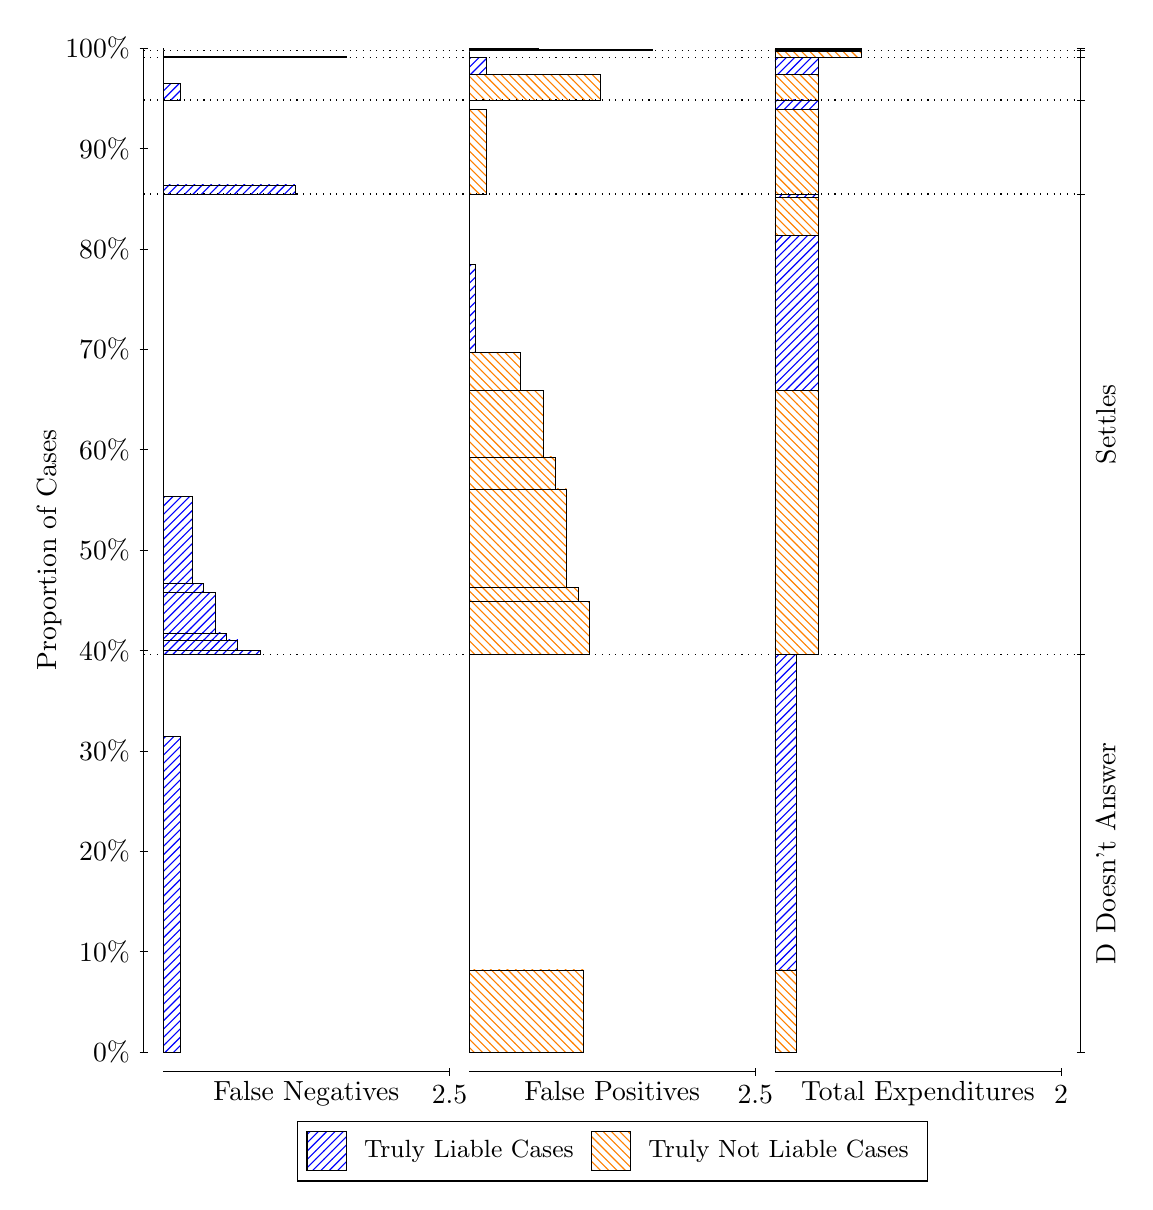
\begin{tikzpicture}
\draw[black, very thin] (1.5,1.75) -- (1.5,14.5);
\node[rotate=90, text=black, anchor=center] at (0.3, 8.125) {Proportion of Cases};
\draw[black, very thin] (1.45,1.75) -- (1.55,1.75);
\node[text=black, anchor=east] at (1.45, 1.75) {0\%};
\draw[black, very thin] (1.45,3.025) -- (1.55,3.025);
\node[text=black, anchor=east] at (1.45, 3.025) {10\%};
\draw[black, very thin] (1.45,4.3) -- (1.55,4.3);
\node[text=black, anchor=east] at (1.45, 4.3) {20\%};
\draw[black, very thin] (1.45,5.575) -- (1.55,5.575);
\node[text=black, anchor=east] at (1.45, 5.575) {30\%};
\draw[black, very thin] (1.45,6.85) -- (1.55,6.85);
\node[text=black, anchor=east] at (1.45, 6.85) {40\%};
\draw[black, very thin] (1.45,8.125) -- (1.55,8.125);
\node[text=black, anchor=east] at (1.45, 8.125) {50\%};
\draw[black, very thin] (1.45,9.4) -- (1.55,9.4);
\node[text=black, anchor=east] at (1.45, 9.4) {60\%};
\draw[black, very thin] (1.45,10.675) -- (1.55,10.675);
\node[text=black, anchor=east] at (1.45, 10.675) {70\%};
\draw[black, very thin] (1.45,11.95) -- (1.55,11.95);
\node[text=black, anchor=east] at (1.45, 11.95) {80\%};
\draw[black, very thin] (1.45,13.225) -- (1.55,13.225);
\node[text=black, anchor=east] at (1.45, 13.225) {90\%};
\draw[black, very thin] (1.45,14.5) -- (1.55,14.5);
\node[text=black, anchor=east] at (1.45, 14.5) {100\%};

\draw[black, very thin] (13.4,1.75) -- (13.4,14.5);
\draw[black, very thin] (13.35,1.75) -- (13.45,1.75);
\node[anchor=west] at (13.35, 1.75) {};
\draw[black, very thin] (13.35,6.8006) -- (13.45,6.8006);
\node[anchor=west] at (13.35, 6.8006) {};
\draw[black, very thin] (13.35,12.646) -- (13.45,12.646);
\node[anchor=west] at (13.35, 12.646) {};
\draw[black, very thin] (13.35,13.84) -- (13.45,13.84);
\node[anchor=west] at (13.35, 13.84) {};
\draw[black, very thin] (13.35,14.381) -- (13.45,14.381);
\node[anchor=west] at (13.35, 14.381) {};
\draw[black, very thin] (13.35,14.469) -- (13.45,14.469);
\node[anchor=west] at (13.35, 14.469) {};
\draw[black, very thin] (13.35,14.5) -- (13.45,14.5);
\node[anchor=west] at (13.35, 14.5) {};

\draw[black, very thin, pattern color=blue, pattern=north east lines] (1.75,1.75) rectangle (1.968,5.7587);
\draw[black, very thin, pattern color=orange, pattern=north west lines] (1.75,5.7587) rectangle (1.75,6.8006);
\draw[black, very thin, pattern color=blue, pattern=north east lines] (1.75,6.8006) rectangle (2.9853,6.8466);
\draw[black, very thin, pattern color=blue, pattern=north east lines] (1.75,6.8466) rectangle (2.6947,6.9824);
\draw[black, very thin, pattern color=blue, pattern=north east lines] (1.75,6.9824) rectangle (2.5493,7.0725);
\draw[black, very thin, pattern color=blue, pattern=north east lines] (1.75,7.0725) rectangle (2.404,7.5848);
\draw[black, very thin, pattern color=blue, pattern=north east lines] (1.75,7.5848) rectangle (2.2587,7.6968);
\draw[black, very thin, pattern color=blue, pattern=north east lines] (1.75,7.6968) rectangle (2.1133,8.8082);
\draw[black, very thin, pattern color=orange, pattern=north west lines] (1.75,8.8082) rectangle (1.75,12.646);
\draw[black, very thin, pattern color=blue, pattern=north east lines] (1.75,12.646) rectangle (3.4213,12.762);
\draw[black, very thin, pattern color=orange, pattern=north west lines] (1.75,12.762) rectangle (1.75,13.84);
\draw[black, very thin, pattern color=blue, pattern=north east lines] (1.75,13.84) rectangle (1.968,14.052);
\draw[black, very thin, pattern color=orange, pattern=north west lines] (1.75,14.052) rectangle (1.75,14.381);
\draw[black, very thin, pattern color=blue, pattern=north east lines] (1.75,14.381) rectangle (4.0753,14.398);
\draw[black, very thin, pattern color=orange, pattern=north west lines] (1.75,14.398) rectangle (1.75,14.469);
\draw[black, very thin, pattern color=orange, pattern=north west lines] (1.75,14.469) rectangle (1.75,14.486);
\draw[black, very thin, pattern color=blue, pattern=north east lines] (1.75,14.486) rectangle (1.75,14.5);
\draw[black, very thin, pattern color=orange, pattern=north west lines] (5.6333,1.75) rectangle (7.0867,2.7919);
\draw[black, very thin, pattern color=blue, pattern=north east lines] (5.6333,2.7919) rectangle (5.6333,6.8006);
\draw[black, very thin, pattern color=orange, pattern=north west lines] (5.6333,6.8006) rectangle (7.1593,7.472);
\draw[black, very thin, pattern color=orange, pattern=north west lines] (5.6333,7.472) rectangle (7.014,7.6489);
\draw[black, very thin, pattern color=orange, pattern=north west lines] (5.6333,7.6489) rectangle (6.8687,8.9014);
\draw[black, very thin, pattern color=orange, pattern=north west lines] (5.6333,8.9014) rectangle (6.7233,9.3072);
\draw[black, very thin, pattern color=orange, pattern=north west lines] (5.6333,9.3072) rectangle (6.578,10.155);
\draw[black, very thin, pattern color=orange, pattern=north west lines] (5.6333,10.155) rectangle (6.2873,10.638);
\draw[black, very thin, pattern color=blue, pattern=north east lines] (5.6333,10.638) rectangle (5.706,11.75);
\draw[black, very thin, pattern color=blue, pattern=north east lines] (5.6333,11.75) rectangle (5.6333,12.646);
\draw[black, very thin, pattern color=orange, pattern=north west lines] (5.6333,12.646) rectangle (5.8513,13.724);
\draw[black, very thin, pattern color=blue, pattern=north east lines] (5.6333,13.724) rectangle (5.6333,13.84);
\draw[black, very thin, pattern color=orange, pattern=north west lines] (5.6333,13.84) rectangle (7.3047,14.169);
\draw[black, very thin, pattern color=blue, pattern=north east lines] (5.6333,14.169) rectangle (5.8513,14.381);
\draw[black, very thin, pattern color=orange, pattern=north west lines] (5.6333,14.381) rectangle (5.6333,14.453);
\draw[black, very thin, pattern color=blue, pattern=north east lines] (5.6333,14.453) rectangle (5.6333,14.469);
\draw[black, very thin, pattern color=orange, pattern=north west lines] (5.6333,14.469) rectangle (7.9587,14.486);
\draw[black, very thin, pattern color=blue, pattern=north east lines] (5.6333,14.486) rectangle (6.5053,14.5);
\draw[black, very thin, pattern color=orange, pattern=north west lines] (9.5167,1.75) rectangle (9.7892,2.7919);
\draw[black, very thin, pattern color=blue, pattern=north east lines] (9.5167,2.7919) rectangle (9.7892,6.8006);
\draw[black, very thin, pattern color=orange, pattern=north west lines] (9.5167,6.8006) rectangle (10.062,10.155);
\draw[black, very thin, pattern color=blue, pattern=north east lines] (9.5167,10.155) rectangle (10.062,12.117);
\draw[black, very thin, pattern color=orange, pattern=north west lines] (9.5167,12.117) rectangle (10.062,12.6);
\draw[black, very thin, pattern color=blue, pattern=north east lines] (9.5167,12.6) rectangle (10.062,12.646);
\draw[black, very thin, pattern color=orange, pattern=north west lines] (9.5167,12.646) rectangle (10.062,13.724);
\draw[black, very thin, pattern color=blue, pattern=north east lines] (9.5167,13.724) rectangle (10.062,13.84);
\draw[black, very thin, pattern color=orange, pattern=north west lines] (9.5167,13.84) rectangle (10.062,14.169);
\draw[black, very thin, pattern color=blue, pattern=north east lines] (9.5167,14.169) rectangle (10.062,14.381);
\draw[black, very thin, pattern color=orange, pattern=north west lines] (9.5167,14.381) rectangle (10.607,14.453);
\draw[black, very thin, pattern color=blue, pattern=north east lines] (9.5167,14.453) rectangle (10.607,14.469);
\draw[black, very thin, pattern color=orange, pattern=north west lines] (9.5167,14.469) rectangle (10.607,14.486);
\draw[black, very thin, pattern color=blue, pattern=north east lines] (9.5167,14.486) rectangle (10.607,14.5);
\draw[black, dotted] (1.5,6.8006) -- (13.4,6.8006);
\draw[black, dotted] (1.5,12.646) -- (13.4,12.646);
\draw[black, dotted] (1.5,13.84) -- (13.4,13.84);
\draw[black, dotted] (1.5,14.381) -- (13.4,14.381);
\draw[black, dotted] (1.5,14.469) -- (13.4,14.469);
\draw[black, very thin] (1.75,1.5) -- (5.3833,1.5);
\node[text=black, anchor=north] at (3.5667, 1.5) {False Negatives};
\draw[black, very thin] (5.3833,1.45) -- (5.3833,1.55);
\node[text=black, anchor=north] at (5.3833, 1.45) {2.5};

\draw[black, very thin] (5.6333,1.5) -- (9.2667,1.5);
\node[text=black, anchor=north] at (7.45, 1.5) {False Positives};
\draw[black, very thin] (9.2667,1.45) -- (9.2667,1.55);
\node[text=black, anchor=north] at (9.2667, 1.45) {2.5};

\draw[black, very thin] (9.5167,1.5) -- (13.15,1.5);
\node[text=black, anchor=north] at (11.333, 1.5) {Total Expenditures};
\draw[black, very thin] (13.15,1.45) -- (13.15,1.55);
\node[text=black, anchor=north] at (13.15, 1.45) {2};

\node[text=black, centered, rotate=90] at (13.72, 4.2753) {D Doesn't Answer};
\node[text=black, centered, rotate=90] at (13.72, 9.7233) {Settles};





\draw (7.449999999999999,1.5) node[draw=none] (baseCoordinate) {};
\begin{scope}[align=center]
        \matrix[scale=0.5, draw=black, below=0.5cm of baseCoordinate, nodes={draw}, column sep=0.1cm]{
            \node[rectangle, draw, minimum width=0.5cm, minimum height=0.5cm, pattern color=blue, pattern=north east lines] {}; &
            \node[draw=none, font=\small, text=black] (B) {Truly Liable Cases}; &
            \node[rectangle, draw, minimum width=0.5cm, minimum height=0.5cm, pattern color=orange, pattern=north west lines] {}; &
            \node[draw=none, font=\small, text=black] (B) {Truly Not Liable Cases}; \\
            };
\end{scope}

\end{tikzpicture}
\end{document}